\documentclass[tikz,border=12pt]{standalone}
\usepackage{amsmath,amssymb,amsfonts}
\usepackage{tikz}
\usetikzlibrary{shapes,arrows.meta,positioning,calc,fit,backgrounds,decorations.pathreplacing,shadows}

% --- Color Palette ---
\definecolor{themeblue}{RGB}{37, 99, 235}
\definecolor{themeteal}{RGB}{13, 148, 136}
\definecolor{themepurple}{RGB}{124, 58, 237}
\definecolor{themeorange}{RGB}{234, 88, 12}
\definecolor{themegreen}{RGB}{22, 163, 74}
\definecolor{themered}{RGB}{220, 38, 38}
\definecolor{themegray}{RGB}{100, 116, 139}
\definecolor{themecyan}{RGB}{6, 182, 212}
\definecolor{themeamber}{RGB}{217, 119, 6}

\begin{document}
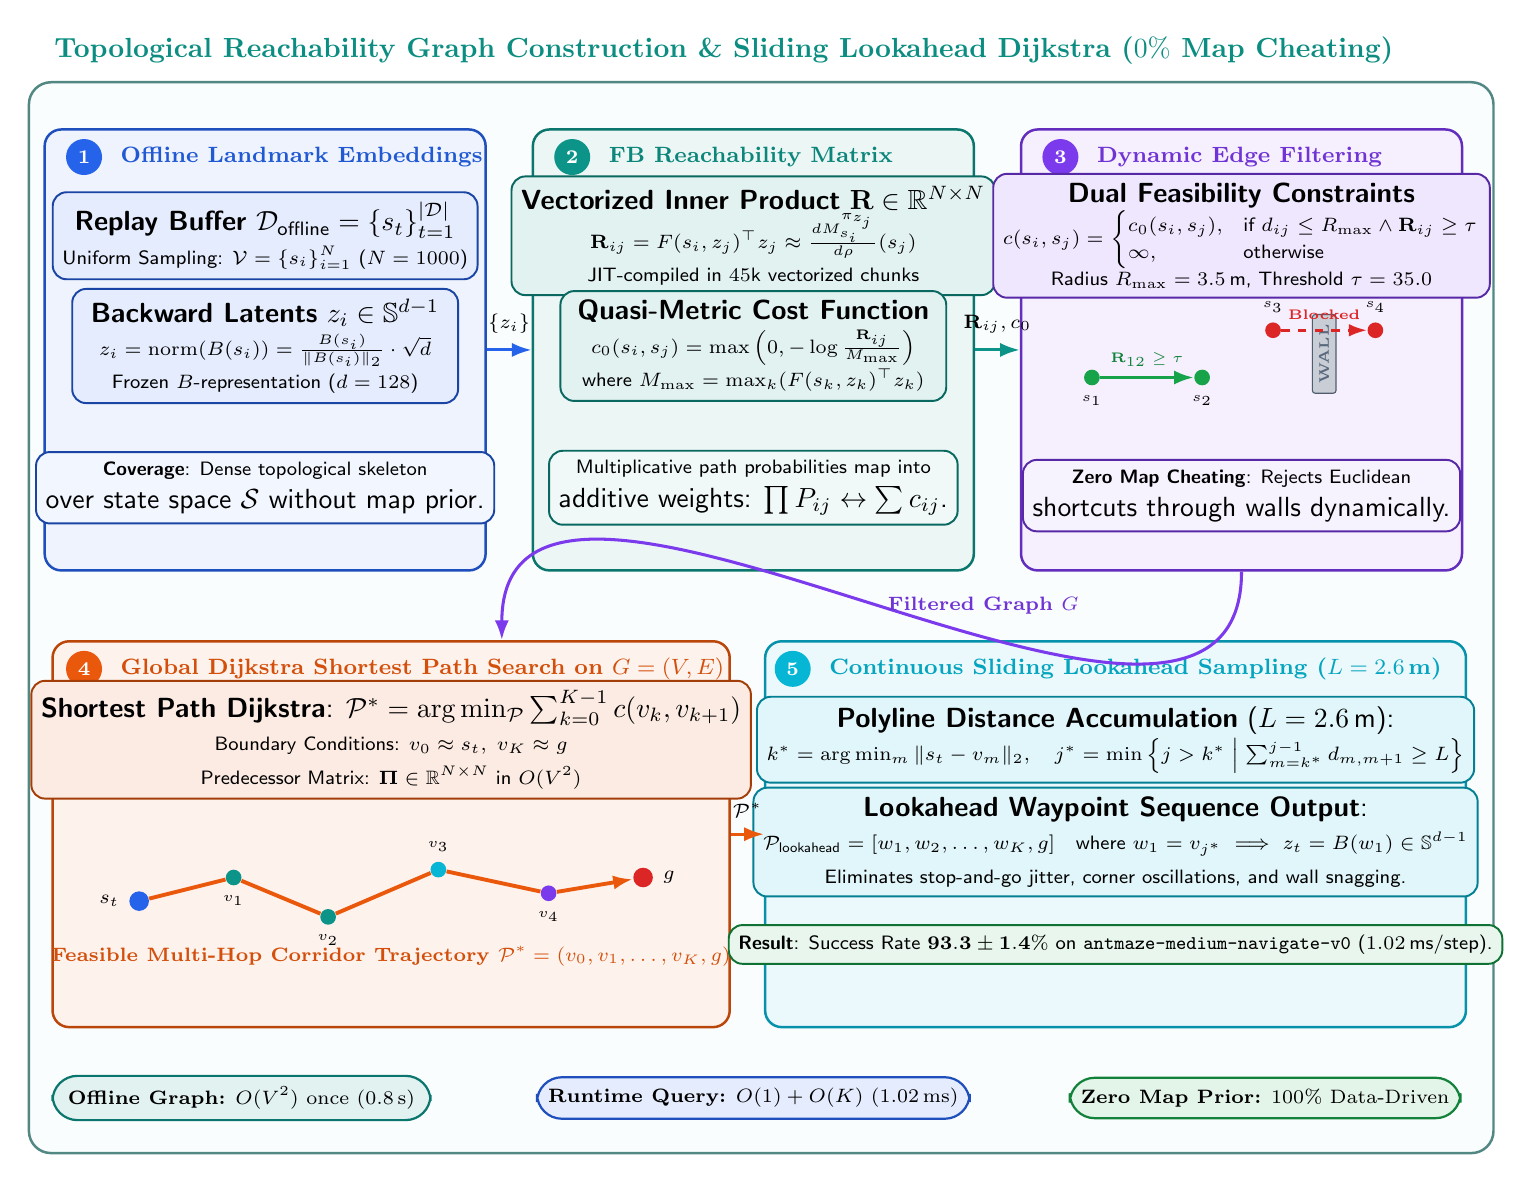
\begin{tikzpicture}[
    >=Latex,
    font=\sffamily,
    % Node styles
    box/.style={
        rectangle,
        rounded corners=6pt,
        draw=#1!80!black,
        fill=#1!8,
        line width=0.9pt,
        align=center,
        inner sep=6pt
    },
    subbox/.style={
        rectangle,
        rounded corners=5pt,
        draw=#1!70!black,
        fill=#1!12,
        line width=0.7pt,
        align=center,
        inner sep=3.5pt
    },
    badge/.style={
        circle,
        fill=#1,
        text=white,
        font=\bfseries\scriptsize,
        inner sep=0.5pt,
        minimum size=13pt
    },
    pill/.style={
        rectangle,
        rounded corners=9pt,
        draw=#1!80!black,
        fill=#1!12,
        line width=0.8pt,
        align=center,
        inner sep=4pt
    },
    arr/.style={
        -{Latex[length=2.5mm,width=1.8mm]},
        line width=1.1pt,
        draw=themegray!80!black
    },
    carr/.style={
        -{Latex[length=2.5mm,width=1.8mm]},
        line width=1.1pt,
        draw=#1
    },
    darr/.style={
        -{Latex[length=2.3mm,width=1.6mm]},
        line width=1.0pt,
        dashed,
        draw=#1
    }
]

% ==============================================================================
% TITLE
% ==============================================================================
\node[anchor=west, font=\bfseries\normalsize, text=themeteal!95!black] at (-0.3, 7.6) 
    {Topological Reachability Graph Construction \& Sliding Lookahead Dijkstra ($0\%$ Map Cheating)};

% Main Enclosing Canvas
\draw[rounded corners=8pt, line width=0.9pt, draw=themeteal!40!gray, fill=themeteal!2] 
    (-0.5, -6.4) rectangle (18.1, 7.2);

% ==============================================================================
% TOP ROW: STEPS 1, 2, 3
% ==============================================================================

% --- Step 1: Landmark Sampling & Latent Embedding ---
\node[box=themeblue, minimum width=5.6cm, minimum height=5.6cm] (card1) at (2.5, 3.8) {};
\node[badge=themeblue] (b1) at (0.2, 6.25) {1};
\node[font=\bfseries\footnotesize, text=themeblue!90!black, right=3pt of b1] {Offline Landmark Embeddings};

\node[subbox=themeblue, minimum width=4.9cm] at (2.5, 5.25) 
    {\textbf{Replay Buffer} $\mathcal{D}_{\text{offline}} = \{s_t\}_{t=1}^{|\mathcal{D}|}$\\\scriptsize Uniform Sampling: $\mathcal{V} = \{s_i\}_{i=1}^N$ ($N=1000$)};

\node[subbox=themeblue, minimum width=4.9cm] at (2.5, 3.85) 
    {\textbf{Backward Latents} $z_i \in \mathbb{S}^{d-1}$\\\scriptsize $z_i = \operatorname{norm}(B(s_i)) = \frac{B(s_i)}{\|B(s_i)\|_2} \cdot \sqrt{d}$\\\scriptsize Frozen $B$-representation ($d=128$)};

\node[subbox=themeblue, fill=themeblue!6, minimum width=4.9cm] at (2.5, 2.05) 
    {\scriptsize \textbf{Coverage}: Dense topological skeleton\\over state space $\mathcal{S}$ without map prior.};


% --- Step 2: Batch Reachability & Log Cost Matrix ---
\node[box=themeteal, minimum width=5.6cm, minimum height=5.6cm] (card2) at (8.7, 3.8) {};
\node[badge=themeteal] (b2) at (6.4, 6.25) {2};
\node[font=\bfseries\footnotesize, text=themeteal!90!black, right=3pt of b2] {FB Reachability Matrix};

\node[subbox=themeteal, minimum width=4.9cm] at (8.7, 5.25) 
    {\textbf{Vectorized Inner Product} $\mathbf{R} \in \mathbb{R}^{N \times N}$\\\scriptsize $\mathbf{R}_{ij} = F(s_i, z_j)^\top z_j \approx \frac{dM^{\pi_{z_j}}_{s_i}}{d\rho}(s_j)$\\
    \scriptsize JIT-compiled in $45\text{k}$ vectorized chunks};

\node[subbox=themeteal, minimum width=4.9cm] at (8.7, 3.85) 
    {\textbf{Quasi-Metric Cost Function}\\\scriptsize $c_0(s_i, s_j) = \max\left(0, -\log \frac{\mathbf{R}_{ij}}{M_{\max}}\right)$\\
    \scriptsize where $M_{\max} = \max_k (F(s_k, z_k)^\top z_k)$};

\node[subbox=themeteal, fill=themeteal!6, minimum width=4.9cm] at (8.7, 2.05) 
    {\scriptsize Multiplicative path probabilities map into\\additive weights: $\prod P_{ij} \leftrightarrow \sum c_{ij}$.};


% --- Step 3: Geometry & Dynamic Edge Filtering ---
\node[box=themepurple, minimum width=5.6cm, minimum height=5.6cm] (card3) at (14.9, 3.8) {};
\node[badge=themepurple] (b3) at (12.6, 6.25) {3};
\node[font=\bfseries\footnotesize, text=themepurple!90!black, right=3pt of b3] {Dynamic Edge Filtering};

\node[subbox=themepurple, minimum width=4.9cm] at (14.9, 5.25) 
    {\textbf{Dual Feasibility Constraints}\\
    \scriptsize $c(s_i, s_j) = \begin{cases} c_0(s_i, s_j), & \text{if } d_{ij} \le R_{\max} \land \mathbf{R}_{ij} \ge \tau \\ \infty, & \text{otherwise} \end{cases}$\\
    \scriptsize Radius $R_{\max} = 3.5\,\text{m}$, Threshold $\tau = 35.0$};

% Visual Mini-Graph of Wall Filtering
\begin{scope}[shift={(12.6, 3.65)}]
    % Corridor Nodes (Valid Edge)
    \node[circle, fill=themegreen, inner sep=2pt, label={[font=\tiny]below:$s_1$}] (n1) at (0.4, -0.2) {};
    \node[circle, fill=themegreen, inner sep=2pt, label={[font=\tiny]below:$s_2$}] (n2) at (1.8, -0.2) {};
    \draw[carr=themegreen, line width=1.2pt] (n1) -- node[above, font=\tiny\bfseries, text=themegreen!80!black] {$\mathbf{R}_{12} \ge \tau$} (n2);
    
    % Wall Barrier & Blocked Edge
    \node[circle, fill=themered, inner sep=2pt, label={[font=\tiny]above:$s_3$}] (n3) at (2.7, 0.4) {};
    \node[circle, fill=themered, inner sep=2pt, label={[font=\tiny]above:$s_4$}] (n4) at (4.0, 0.4) {};
    \draw[fill=themegray!35, draw=themegray!80!black, rounded corners=1pt] (3.2, -0.4) rectangle (3.5, 0.6);
    \node[font=\tiny\bfseries, text=themegray!90!black, rotate=90] at (3.35, 0.1) {WALL};
    \draw[darr=themered, line width=1.0pt] (n3) -- node[above, font=\tiny\bfseries, text=themered] {Blocked} (n4);
\end{scope}

\node[subbox=themepurple, fill=themepurple!6, minimum width=4.9cm] at (14.9, 1.95) 
    {\scriptsize \textbf{Zero Map Cheating}: Rejects Euclidean\\shortcuts through walls dynamically.};


% ==============================================================================
% BOTTOM ROW: STEPS 4, 5 & SAMPLING WORKFLOW
% ==============================================================================

% --- Step 4: Global Dijkstra Search ---
\node[box=themeorange, minimum width=8.6cm, minimum height=4.9cm] (card4) at (4.1, -2.35) {};
\node[badge=themeorange] (b4) at (0.2, -0.25) {4};
\node[font=\bfseries\footnotesize, text=themeorange!90!black, right=3pt of b4] {Global Dijkstra Shortest Path Search on $G=(V, E)$};

\node[subbox=themeorange, minimum width=8.0cm] at (4.1, -1.15) 
    {\textbf{Shortest Path Dijkstra}: $\mathcal{P}^* = \arg\min_{\mathcal{P}} \sum_{k=0}^{K-1} c(v_k, v_{k+1})$\\
    \scriptsize Boundary Conditions: $v_0 \approx s_t, \; v_K \approx g$\\
    \scriptsize Predecessor Matrix: $\mathbf{\Pi} \in \mathbb{R}^{N \times N}$ in $O(V^2)$};

% Visual Path Polyline
\begin{scope}[shift={(0.6, -3.2)}]
    \node[circle, fill=themeblue, inner sep=2.5pt, label={[font=\scriptsize\bfseries]left:$s_t$}] (p0) at (0.3, 0) {};
    \node[circle, fill=themeteal, inner sep=2pt, label={[font=\tiny]below:$v_1$}] (p1) at (1.5, 0.3) {};
    \node[circle, fill=themeteal, inner sep=2pt, label={[font=\tiny]below:$v_2$}] (p2) at (2.7, -0.2) {};
    \node[circle, fill=themecyan, inner sep=2pt, label={[font=\tiny]above:$v_3$}] (p3) at (4.1, 0.4) {};
    \node[circle, fill=themepurple, inner sep=2pt, label={[font=\tiny]below:$v_4$}] (p4) at (5.5, 0.1) {};
    \node[circle, fill=themered, inner sep=2.5pt, label={[font=\scriptsize\bfseries]right:$g$}] (p5) at (6.7, 0.3) {};
    
    \draw[carr=themeorange, line width=1.4pt] (p0) -- (p1) -- (p2) -- (p3) -- (p4) -- (p5);
    \node[font=\scriptsize\bfseries, text=themeorange!90!black] at (3.5, -0.7) {Feasible Multi-Hop Corridor Trajectory $\mathcal{P}^* = (v_0, v_1, \dots, v_K, g)$};
\end{scope}


% --- Step 5: Continuous Sliding Lookahead ---
\node[box=themecyan, minimum width=8.9cm, minimum height=4.9cm] (card5) at (13.3, -2.35) {};
\node[badge=themecyan] (b5) at (9.2, -0.25) {5};
\node[font=\bfseries\footnotesize, text=themecyan!90!black, right=3pt of b5] {Continuous Sliding Lookahead Sampling ($L = 2.6\,\text{m}$)};

\node[subbox=themecyan, minimum width=8.2cm] at (13.3, -1.15) 
    {\textbf{Polyline Distance Accumulation} ($L = 2.6\,\text{m}$):\\
    \scriptsize $k^* = \arg\min_m \|s_t - v_m\|_2, \quad j^* = \min \left\{ j > k^* \;\middle|\; \sum_{m=k^*}^{j-1} d_{m,m+1} \ge L \right\}$};

\node[subbox=themecyan, minimum width=8.2cm] at (13.3, -2.45) 
    {\textbf{Lookahead Waypoint Sequence Output}:\\
    \scriptsize $\mathcal{P}_{\text{lookahead}} = [w_1, w_2, \dots, w_K, g] \quad \text{where } w_1 = v_{j^*} \implies z_t = B(w_1) \in \mathbb{S}^{d-1}$\\
    \scriptsize Eliminates stop-and-go jitter, corner oscillations, and wall snagging.};

\node[subbox=themegreen, fill=themegreen!10, minimum width=8.2cm] at (13.3, -3.75) 
    {\scriptsize \textbf{Result}: Success Rate $\mathbf{93.3 \pm 1.4\%}$ on \texttt{antmaze-medium-navigate-v0} ($1.02\,\text{ms}$/step).};


% ==============================================================================
% CONNECTING ARROWS BETWEEN PANELS
% ==============================================================================
\draw[carr=themeblue] (card1.east) -- node[above=2pt, font=\scriptsize\bfseries] {$\{z_i\}$} (card2.west);
\draw[carr=themeteal] (card2.east) -- node[above=2pt, font=\scriptsize\bfseries] {$\mathbf{R}_{ij}, c_0$} (card3.west);
\draw[carr=themepurple] (card3.south) to[out=270, in=90] node[midway, right=2pt, font=\scriptsize\bfseries, text=themepurple!90!black] {Filtered Graph $G$} ([xshift=40pt]card4.north);
\draw[carr=themeorange] (card4.east) -- node[above=2pt, font=\scriptsize\bfseries] {$\mathcal{P}^*$} (card5.west);


% ==============================================================================
% BOTTOM SUMMARY PILLS
% ==============================================================================
\node[pill=themeteal, font=\scriptsize, minimum width=4.8cm] at (2.2, -5.7) 
    {\textbf{Offline Graph:} $O(V^2)$ once ($0.8\,\text{s}$)};

\node[pill=themeblue, font=\scriptsize, minimum width=4.8cm] at (8.7, -5.7) 
    {\textbf{Runtime Query:} $O(1) + O(K)$ ($1.02\,\text{ms}$)};

\node[pill=themegreen, font=\scriptsize, minimum width=4.8cm] at (15.2, -5.7) 
    {\textbf{Zero Map Prior:} 100\% Data-Driven};

\end{tikzpicture}
\end{document}
